\chapter{Hardware:}
\section{Raspberry Pi 3}{
	\begin{figure}[H]
		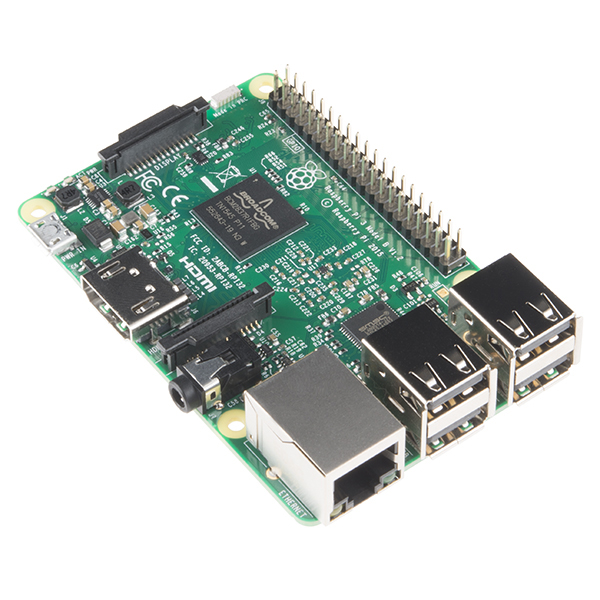
\includegraphics[scale=2]{images/rpi.jpg}
		\centering
		% first figure itself
		\caption{Raspberry Pi 3}
		\label{trans}
	\end{figure}
	The Raspberry Pi 3 is the third generation Raspberry Pi. This powerful
    credit-card sized single board computer can be used for many applications
    and supersedes the Raspberry Pi 2 Model. Whilst maintaining the popular board format the Raspberry Pi 3 Model
    B brings you a more powerful processer, 10x faster than the first generation
    Raspberry Pi. Additionally it adds wireless LAN & Bluetooth connectivity
    making it the ideal solution for powerful connected designs. It has a HDMI (rev 1.3 & 1.4 Composite RCA (PAL and NTSC).It uses Broadcom BCM2387 chipset with a
    1.2GHz Quad-Core ARM Cortex-A53 and 802.11 b/g/n Wireless LAN and Bluetooth 4.1 (Bluetooth Classic and LE). It also has a 1GB LPDDR2 memory. Operating System Boots from Micro SD card, running a version of the Linux operating system or
    Windows 10 IoT.
	%\begin{equation}
	%	C = 0.7 \times I /(\Delta V \times F)
	%\end{equation}
	
}
\section{ACS712 Module Current Sensor}{
	\begin{figure}[H]
	    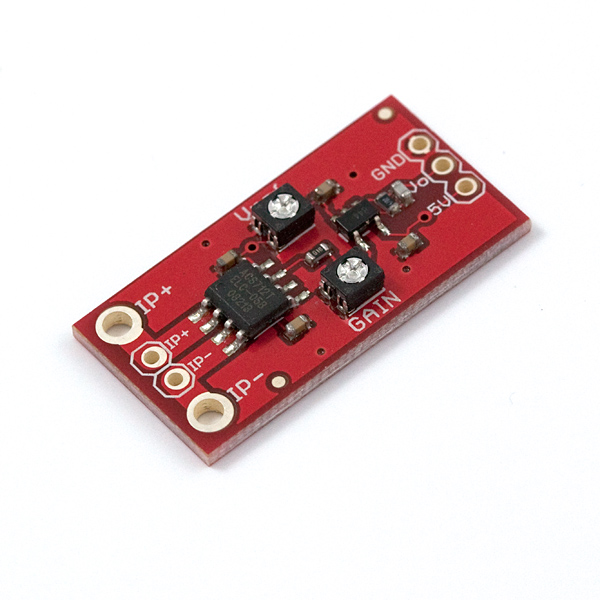
\includegraphics[scale=0.5]{images/acs712.jpg}
	    \centering
	    \caption{ACS712}
	    \label{ACS712}
	\end{figure}
	
	\begin{figure}[H]
	    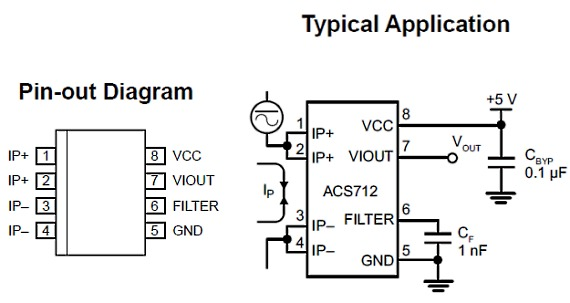
\includegraphics[scale=0.75]{PinDiagrams.jpg}
	    \centering
	    \caption{ACS712 Block Diagram}
	    \label{fig:my_label}
	\end{figure}
	The Allegro ACS712 provides economical and precise solutions for AC or DC current sensing in industrial, commercial, and communications systems.The device consists of a precise, low-offset, linear Hall circuit with a copper conduction path located near the surface of the die. Applied current flowing through this copper conduction path generates a magnetic field which the Hall IC converts into a proportional voltage. Device accuracy is optimized through the close proximity of the magnetic signal to the Hall transducer. A precise, proportional voltage is provided by the low-offset, chopper-stabilized BiCMOS Hall IC, which is programmed for accuracy after packaging. The internal resistance of this conductive path is 1.2 mΩ typical, providing low power loss. The thickness of the copper conductor allows survival of the device at up to 5× overcurrent conditions. The terminals of the conductive path are electrically isolated from the signal leads (pins 5 through 8). This allows the ACS712 to be used in applications requiring electrical isolation without the use of opto-isolators or other costly isolation techniques. It requires a 4.5-5.5V power supply. It takes input current of 0-30A and produces output voltage of 2.5-5V.
}

\section{ADC ADS1115}{
\begin{figure}[H]
		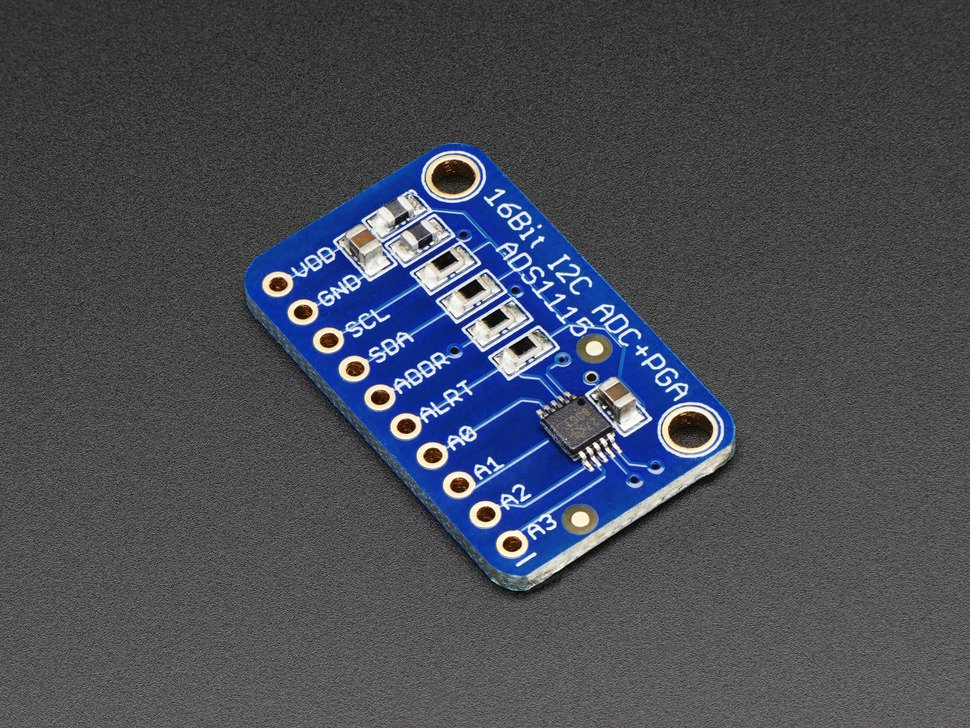
\includegraphics[scale=0.5]{images/ads1115.jpg}
		\centering
		% first figure itself
		\caption{Raspberry Pi 3}
		\label{trans}
	\end{figure}

For microcontrollers without an analog-to-digital converter or when you want a higher-precision ADC, the ADS1115 provides 16-bit precision at 860 samples/second over I2C. The chip can be configured as 4 single-ended input channels, or two differential channels. As a nice bonus, it even includes a programmable gain amplifier, up to x16, to help boost up smaller single/differential signals to the full range. We like this ADC because it can run from 2V to 5V power/logic, can measure a large range of signals and its super easy to use. It is a great general purpose 16 bit converter.

The chip's fairly small so it comes on a breakout board with ferrites to keep the AVDD and AGND quiet. Interfacing is done via I2C. The address can be changed to one of four options so you can have up to 4 ADS1115's connected on a single 2-wire I2C bus for 16 single ended inputs.

}
\section{Current Transformer}{

\begin{figure}[H]
	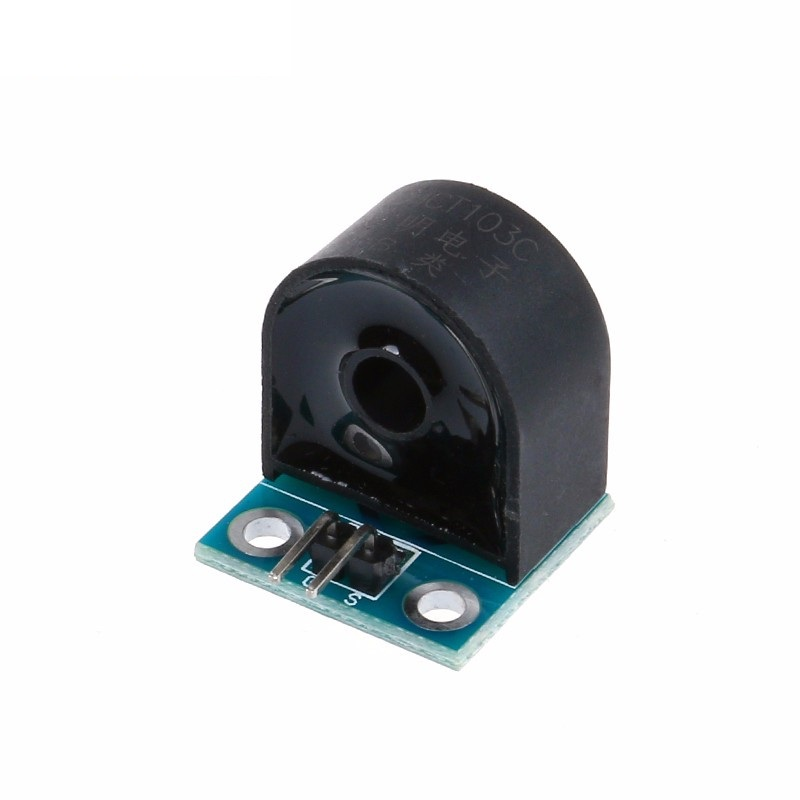
\includegraphics[scale=0.45]{images/CT2.jpg}
	\centering
	
	% first figure itself
	\caption{Current Transformer}
	\label{Current Transformer}
\end{figure}
Current transformers can perform circuit control, measure current for power measurement and control, and perform roles for safety protection and current limiting. They can also cause circuit events to occur when the monitored current reaches a specified level. Current monitoring is necessary at frequencies from the 50 Hz/60 Hz power line to the higher frequencies of switchmode transformers that range into the hundreds of kilohertz.

The object with current transformers is to think in terms of current transformation rather than voltage ratios. Current ratios are the inverse of voltage ratios. The thing to remember about transformers is that Pout = (Pin — transformer power losses). With this in mind, let's assume we had an ideal loss-less transformer in which Pout = Pin. Since power is voltage times current, this product must be the same on the output as it is on the input. This implies that a 1:10 step-up transformer with the voltage stepped up by a factor of 10 results in an output current reduced by a factor of 10. This is what happens on a current transformer. If a transformer had a one-turn primary and a ten-turn secondary, each amp in the primary results in 0.1A in the secondary, or a 10:1 current ratio. It's exactly the inverse of the voltage ratio — preserving volt times current product.

How can we use this transformer and knowledge to produce something useful? Normally, an engineer wants to produce an output on the secondary proportional to the primary current. Quite often, this output is in volts output per amp of primary current. The device that monitors this output voltage can be calibrated to produce the desired results when the voltage reaches a specified level.

A burden resistor connected across the secondary produces an output voltage proportional to the resistor value, based on the amount of current flowing through it. With our 1:10 turns ratio transformer that produces a 10:1 current ratio, a burden resistor can be selected to produce the voltage we want. If 1A on the primary produces 0.1A on the secondary, then by Ohm's law, 0.1 times the burden resistor will result in an output voltage per amp.

Many voltage transformers have adjusted ratios that produce the desired output voltage and compensate for losses. The turns-ratios or actual turns aren't the primary concern of the end-user. Only the voltage output and possibly regulation and other loss parameters may be of concern. With current transformers, the user must know the current ratio to use the transformer. The knowledge of amps in per amps out is the basis for use of the current transformer. Quite often, the end users provide the primary with a wire through the center of the transformer. They must know what secondary turns are to determine what their output current will be. Generally, in catalogues, the turns of the transformers are provided as a specification for use.

With this knowledge, the user can choose the burden resistor to produce their desired output voltage. The output current of 0.1A for a 1A primary on the 1:10 turns ratio transformer will produce 0.1 V/A across a 1Ω burden resistor, 1V per amp across a 10Ω burden and 10V per amp across a 100Ω burden resistor.

The Smart Energy Monitor uses a Current Transformer with a 1:1000 turns ratio & a burden resistor of 40 Ohm.
}

\section{Voltage Transformer}{

\begin{figure}[H]
	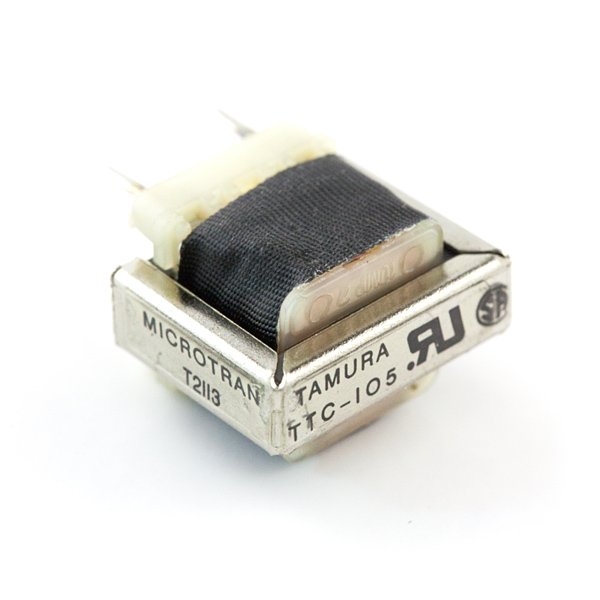
\includegraphics[width=0.9\textwidth]{images/vt.jpg} % first figure itself
	\caption{Voltage Transformer}
	\label{Voltage Transformer}
\end{figure}
Voltage transformers (VT), also called potential transformers (PT), are a parallel connected type of instrument transformer. They are designed to present negligible load to the supply being measured and have an accurate voltage ratio and phase relationship to enable accurate secondary connected metering.
The Smart Energy Monitor uses a 230:5 turns ratio voltage transformer 
}


\section{Arduino}{
\begin{figure}[H]
	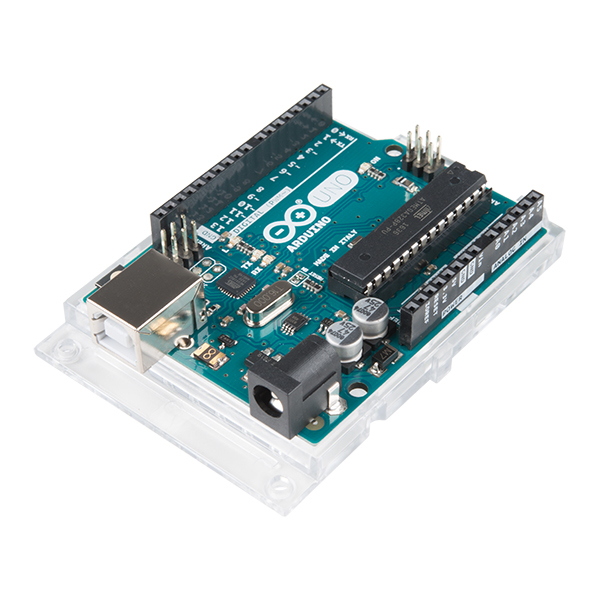
\includegraphics[width=0.9\textwidth]{images/arduino.jpg} % first figure itself
	\caption{Arduino Uno}
	\label{Arduino Uno}
\end{figure}
Arduino Uno is a microcontroller board based on the ATmega328P (datasheet). It has 14 digital input/output pins (of which 6 can be used as PWM outputs), 6 analog inputs, a 16 MHz quartz crystal, a USB connection, a power jack, an ICSP header and a reset button. 
}

\section{Comparator LM339}
{The LM339 devices consist of four independent voltage comparators that are designed to operate from a single power supply over supplies also is possible, as long as the difference between the two supplies is 2 V to 36 V, and VCC isat least 1.5 V more positive than the input common-mode voltage. Current drain is independent of the supply voltage. The outputs can be connected to the other open-collector outputs to achieve wired-AND relationships} 


\section{Operational Amplifier LM324}
{The LM324-N series consists of four independent,
high-gain, internally frequency compensated
operational amplifiers designed to operate from a
single power supply over a wide range of voltages.
Operation from split-power supplies is also possible
and the low-power supply current drain is
independent of the magnitude of the power supply
voltage.}

\section{ExOR Gate 74HC86}
{
The 74HC86 is a quad 2-input EXCLUSIVE-OR gate. Inputs include clamp diodes. This enables the use of current limiting resistors to interface inputs to voltages in excess of VCC. 
}

\chapter{Design and Implementation:}

\section{Current Difference}
{
Inorder to measure the AC Current using the current transformer we must:

\begin{enumerate}
  \item Connect only the Live wire between the AC source and the load appliances through the current transformer.
  \item Measure the peak voltage dropped across the 40 ohm burden resistor that is on the transformer output
  \item Convert that voltage across the resistor to a current by applying ohms law (I = V/R).
  \item Multiply the peak voltage by 0.707 to get and RMS Voltage across the resistor.  (0.707 as a factor only applies to Sine Waves).
  \item Multiply the RMS current by 1000 to get yield the value going through the wire being measured.  (The current transformer has a 1000 to 1 ratio).
  
\end{enumerate}

\begin{figure}[H]
	    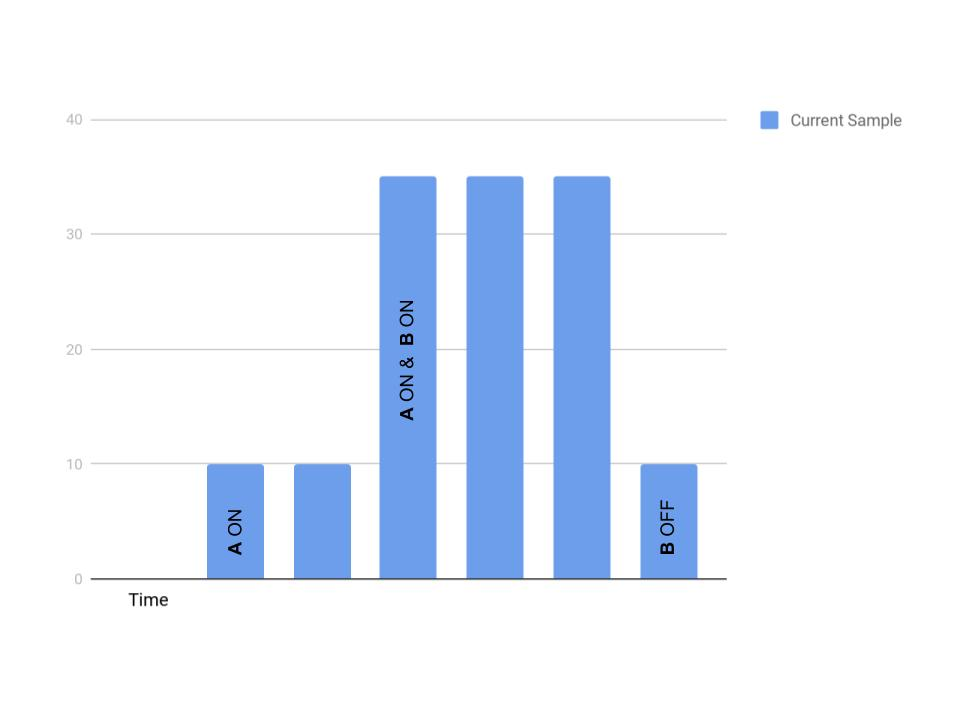
\includegraphics[scale=0.50]{images/cdiff.jpg}
	    \centering
	    \caption{Change in Current between Conscutive Samples}
	    \label{cdiff}
	\end{figure}
	

The Current drawn by the load is the first parameter used to classify the various load appliances. The current transformer is used as a current sensor which will provide us with the instantaneous value of the total current drawn by all loads connected to the Smart Energy Monitor. 
In order to get the value of the current drawn by each individual load appliance we must calculate the difference between each of the consecutive current sample. 

As shown in the above figure, we can see that when load appliance A is turned ON, the change in current is 10, when B is turned ON after A, the change in current is 25 but the total current is 35 and finally when B is turned OFF the change in current is 25 while the total current drawn is 10.

\subsection{Averaging Consecutive Current Samples}
The total change in current that occurs when a load appliance is switched ON/OFF may not be correctly reflected between the two consecutive samples. Instead the total change in current may be reflected over more than two consecutive current samples depending on the switching speed or transient time of the load appliances. Hence, occasionally large errors are produced when measuring the current difference between any two consecutive current samples.

In order to reduce the error, the sampling rate may be adjusted accordingly. But calibrating the sampling rate may be difficult as various load appliances have different transient times as well as the time taken for different software instructions may differ with different hardware and sensors.

\centering
T_{otal} C_{urrent} =  \sum_{0}^{N}C_{urrent} S_{amples}

\begin{figure}[H]
	    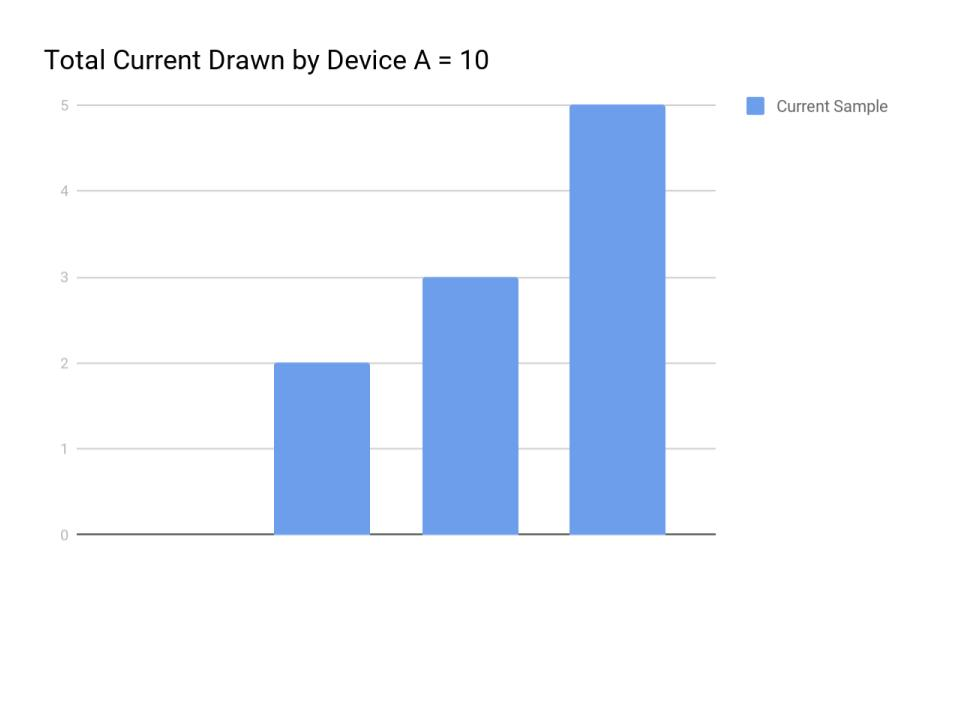
\includegraphics[scale=0.50]{images/cdiff2.jpg}
	    \centering
	    \caption{Sum of N Current Samples}
	    \label{cdiff}
	\end{figure}


A more efficient method for reducing this error will be to find the sum of N consecutive current samples such that the sum of all the error is zero(or close to zero). The user may have to wait for a very short duration before the next load appliance can be switched ON/OFF. The small error that remains will not come into effect as the classification algorithm will rule it out based on the mean and standard deviation values of all the labelled data.

As shown in the above figure, load appliance A during its transient state as a total current change of 10. But this value is not reflected between any two consecutive current samples. Instead the change in current observed between any two consecutive current samples for load appliance A is 2,3 and 5 respectively. Hence the value of error produced will be either 3 or 5. But if we take the sum of N consecutive samples where in N in this case is equal to 3, then we will get an error value of 0.
}

\section{Active Power and Reactive Power}
{
Using only the current drawn by a load as a classification parameter has the following limitation:
\begin{itemize}
  \item If two or more completely different load appliances(different applications) draw the same amount of current, the current difference between N consecutive samples for both the devices may be equal which may produce an incorrect result.
 \end{itemize}
 
 \begin{figure}[H]
	    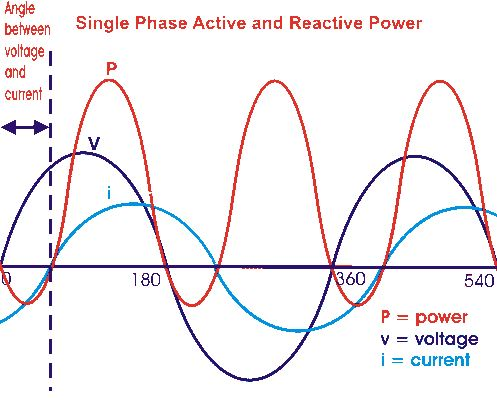
\includegraphics[scale=1]{images/phasediff.JPG}
	    \centering
	    \caption{Phase Difference between Voltage and Current}
	    \label{cdiff}
	\end{figure}

 
 Hence in order to more accurately differentiate between load appliances which draw the same amount of current, we also consider the value of active power and reactive power drawn by each individual load appliance. It will be highly unlikely that two completely different load appliances with different applications and uses have the same current drawn as well as Active Power and Reactive Power values.
}

\section{Phase Angle}
{

\begin{figure}[H]
	    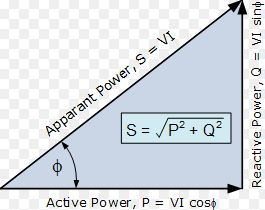
\includegraphics[scale=1]{images/triangle.jpg}
	    \centering
	    \caption{Power Triangle}
	    \label{cdiff}
	\end{figure}

\begin{equation}
    Active\ Power = P = V_{RMS}I_{RMS}\cos\phi
\end{equation}


\begin{equation}
    Reactive\ Power = Q = V_{RMS}I_{RMS}\sin\phi
\end{equation}

\begin{equation}
    Apparent\ Power = S = \sqrt{P^{2}+Q^{2}}
\end{equation}

In order to calculate the Active Power and Reactive Power drawn by load appliances, we must first find the phase difference between the voltage and current.
We do this by implementing a zero cross detector for both the voltage and current. 


\begin{figure}[H]
	    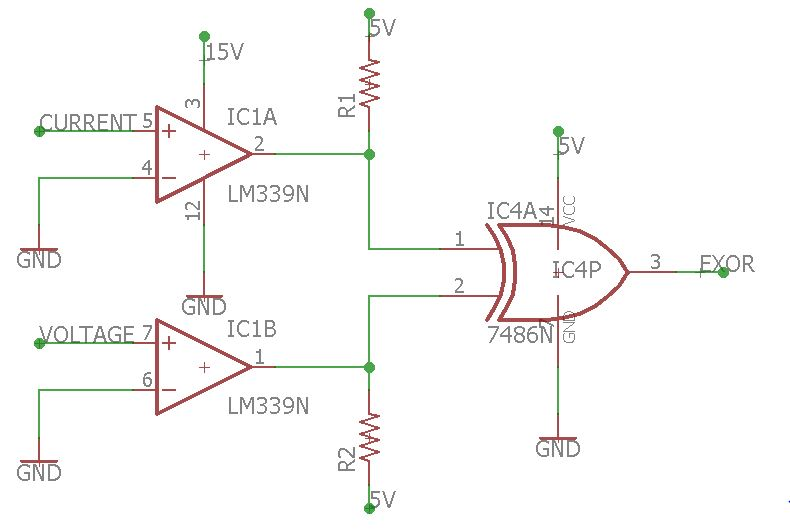
\includegraphics[scale=0.75]{images/zcd.jpg}
	    \centering
	    \caption{Zero Cross Detector}
	    \label{zcd}
	\end{figure}


The zero cross detector is built using the LM339. 

\begin{equation}
    Y = (Voltage + Current) \cdot (\overline{Voltage}+\overline{Current})
\end{equation}

The output of the zero cross detectors is fed to the Ex-OR gate of the 7486 EXOR IC which will produce pulses when there is a phase shift. i.e. The two logic levels of the inputs to the EXOR gate are not equal to each other. 

\begin{equation}
    Phase\ Angle = \phi=360\times Frequency\times \triangle Time
\end{equation}

The time period(t) of these pulses can be be used to find the phase angle between the voltage and current waveforms.

\subsection{Current Amplification}
The current transformer has a turns ratio of 1:1000. Hence if the current drawn by the load is around 1A, the output of the current transformer will be 1mA. Many load appliances draw currents far lower than 1A and hence the resulting voltage developed across the burden resistor connected to the current transformer may be lower than the input common mode voltage of the comparator. 


\begin{figure}[H]
	    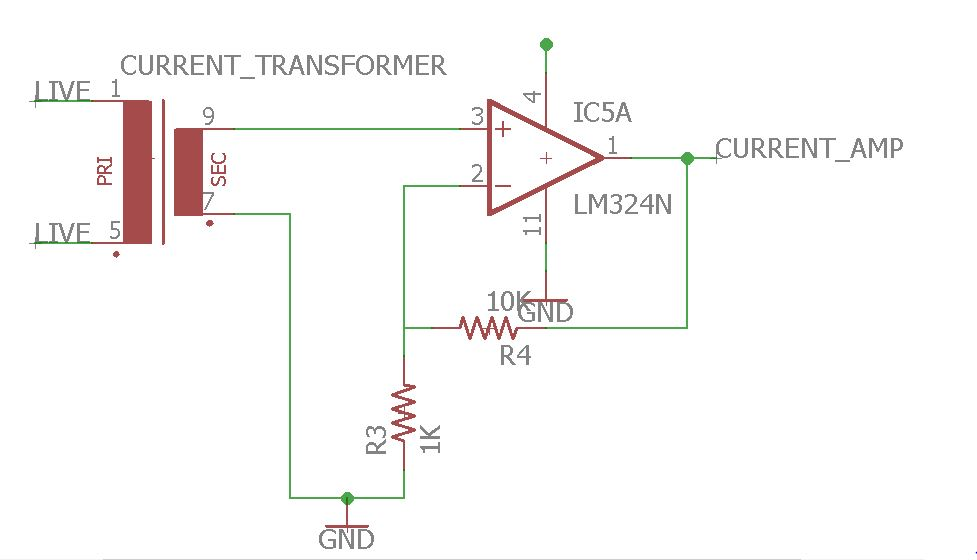
\includegraphics[scale=0.70]{images/iamp.jpg}
	    \centering
	    \caption{Current Signal Amplifier}
	    \label{iamp}
	\end{figure}


In order to produce a voltage that is greater than the input common mode voltage of the comparator, output voltage across the burden resistor must be amplified. A non inverting amplifier must be used so that there is no effect on the values of phase angle between voltage and current.

\begin{equation}
Gain = 1+ \frac{R_{f}}{R_{1}} 
\end{equation}

The LM324 has an operational amplifier which can be configured as an Non Inverting amplifier with suitable gain for the purpose of amplifying the current signal. 
}
\section{Serial Communication}
{
The Arduino is used as a low cost ADC which can transmit data to the Raspberry Pi.
The Arduino transmits this data using Serial Communication through a USB cable. This is useful since no logic level conversion is required when compared to the I2C or GPIO communication protocols.
Data such as the current drawn as well as Active Power and Reactive Power are sent to the Raspberry Pi.
The Arduino is directly powered through its USB port. Hence no additional external power supply is required for the Arduino.


}

\section{Naive Bayes Classification}
{
The Naive Bayes algorithm is an intuitive method that uses the probabilities of each attribute belonging to each class to make a prediction. It is the supervised learning approach you would come up with if you wanted to model a predictive modeling problem probabilistically.

Naive bayes simplifies the calculation of probabilities by assuming that the probability of each attribute belonging to a given class value is independent of all other attributes. This is a strong assumption but results in a fast and effective method.

The probability of a class value given a value of an attribute is called the conditional probability. By multiplying the conditional probabilities together for each attribute for a given class value, we have a probability of a data instance belonging to that class.

To make a prediction we can calculate probabilities of the instance belonging to each class and select the class value with the highest probability.

Naive bases is often described using categorical data because it is easy to describe and calculate using ratios. A more useful version of the algorithm for our purposes supports numeric attributes and assumes the values of each numerical attribute are normally distributed (fall somewhere on a bell curve). Again, this is a strong assumption, but still gives robust results.
}

\subsection{Creating the Dataset}{
The dataset is created by measuring the values of the current drawn, active power and reacive power drawn by individual load appliances. These data points are then used to identify the device.
The change in these parameters must follow the following condition to be considered as valid data point:
\begin{itemize}
    \item The increase in any classification parameter(current drawn, active power and reactive power drawn) when a load appliance is turned ON must be equal to decrease in that classification parameter when the load appliance is turned OFF.
    \item The values of the data points of a particular load appliance must remain the same even if other devices are active. This must apply for all combinations of load appliances and their individual states.
\end{itemize}

The valid data points have to be labelled according to the load appliance state. 
The data is stored in a standard CSV format table.
The more validated & labelled data within the dataset will make the predicted result more accurate. 

}

\subsection{Impelementation of Classification Algorithm}{
The implementation of most classification algorithms involve the following processes:

\begin{enumerate}
  \item \textbf{Handle Data:} Load the data from CSV file and split it into training and test datasets. Split the data into a training dataset that Naive Bayes can use to make predictions and a test dataset that we can use to evaluate the accuracy of the model. 
  
  \begin{equation}
      Training\ Data = 0.67 \times Dataset\ Size
  \end{equation}
  
   \begin{equation}
      Testing\ Data = 0.33 \times Dataset\ Size
  \end{equation}
 
  
  
  We need to split the data set randomly into train and datasets with a ratio of 67 percent train and 33 percent test (this is a common ratio for testing an algorithm on a dataset).


 \item \textbf{Summarize Data: } Summarize the properties in the training dataset so that we can calculate probabilities and make predictions.
 \item \textbf{Make a Prediction:} Use the summaries of the dataset to generate a single prediction.
 \item \textbf{Make Test Data Predictions:} Generate predictions given a test dataset and a summarized training dataset.
\item \textbf{Evaluate Accuracy:} Evaluate the accuracy of predictions made for a test dataset as the percentage correct out of all predictions made.
\item \textbf{Tie it Together:} Use all of the code elements to present a complete and standalone implementation of the Naive Bayes algorithm.
 
\end{enumerate}
}


\subsection{Data Summarizing}{
The naive bayes model is comprised of a summary of the data in the training dataset. This summary is then used when making predictions.

The summary of the training data collected involves the mean and the standard deviation for each attribute, by class value.

These are required when making predictions to calculate the probability of specific attribute values belonging to each class value.

We can break the preparation of this summary data down into the following sub-tasks:

\begin{enumerate}
    \item \textbf{Separate Data By Class:} The first task is to separate the training dataset instances by class value so that we can calculate statistics for each class. We can do that by creating a map of each class value to a list of instances that belong to that class and sort the entire dataset of instances into the appropriate lists.
\item \textbf{Calculate Mean:} We need to calculate the mean of each attribute for a class value.

\begin{equation}
Mean\ of\ each\ Attribute\ for\ Class\ Value = \frac{Sum\ of\ all\ Attributes}{Total\ Number\ of\ Attributes}
\end{equation}

The mean is the central middle or central tendency of the data, and we will use it as the middle of our gaussian distribution when calculating probabilities.

We also need to calculate the standard deviation of each attribute for a class value. The standard deviation describes the variation of spread of the data, and we will use it to characterize the expected spread of each attribute in our Gaussian distribution when calculating probabilities.

\begin{equation}
    Standard\ Deviation\ of\ each\ Attribute\ for\ Class\ Value = \sigma = \sqrt{\frac{\sum_0^n (x-\overline{Mean})^{2}}{n}}
\end{equation}

In the above equation n = The number of attributes.
The standard deviation is calculated as the square root of the variance. The variance is calculated as the average of the squared differences for each attribute value from the mean. 

\item \textbf{Summarize Dataset:} Now we have the tools to summarize a dataset. For a given list of instances (for a class value) we can calculate the mean and the standard deviation for each attribute.

\item \textbf{Summarize Dataset:} Now we have the tools to summarize a dataset. For a given list of instances (for a class value) we can calculate the mean and the standard deviation for each attribute.

\item \textbf{Summarize Attributes By Class:} We can pull it all together by first separating our training dataset into instances grouped by class. Then calculate the summaries for each attribute. 


\end{enumerate}

}

\subsection{Making Predictions}
We are now ready to make predictions using the summaries prepared from our training data. Making predictions involves calculating the probability that a given data instance belongs to each class, then selecting the class with the largest probability as the prediction.

We can divide this part into the following tasks:

\begin{enumerate}
    \item \textbf{Calculate Gaussian Probability Density Function:} We can use a Gaussian function to estimate the probability of a given attribute value, given the known mean and standard deviation for the attribute estimated from the training data.


\begin{equation}
    Gaussian\ Probability = \frac{1}{\sqrt{2\pi \sigma^{2}}} \times Exponent
\end{equation}

\begin{equation}
    Exponent = e^{-\frac{(x-Mean)^{2}}{2 \sigma^{2}}}
\end{equation}



Given that the attribute summaries where prepared for each attribute and class value, the result is the conditional probability of a given attribute value given a class value. 

\item \textbf{Calculate Class Probabilities:} Now that we can calculate the probability of an attribute belonging to a class, we can combine the probabilities of all of the attribute values for a data instance and come up with a probability of the entire data instance belonging to the class.

We combine probabilities together by multiplying them. 

\item \textbf{Making a Prediction:}
Now that can calculate the probability of a data instance belonging to each class value, we can look for the largest probability and return the associated class.
Finally, we can estimate the accuracy of the model by making predictions for each data instance in our test dataset. This will return a list of predictions for each test instance.


\item \textbf{Estimating Accuracy:} 

\begin{equation}
Accuracy = \frac{Number\ of\ Accurate\ Predictions}{Size\ of\ the\ Testing\ Dataset}\times100
\end{equation}

The predictions can be compared to the class values in the test dataset and a classification accuracy can be calculated as an accuracy ratio between 0& and 100%.

\end{enumerate}



\section{Additional Classification Parameters}
The more number of parameters used in classification algorithms will further improve the quality of the dataset.

These additional parameters are non numerical values. Hence a decision tree algorithm along with a Naive Bayes classification must be implemented when considering any non numerical parameters.

\begin{figure}[H]
	    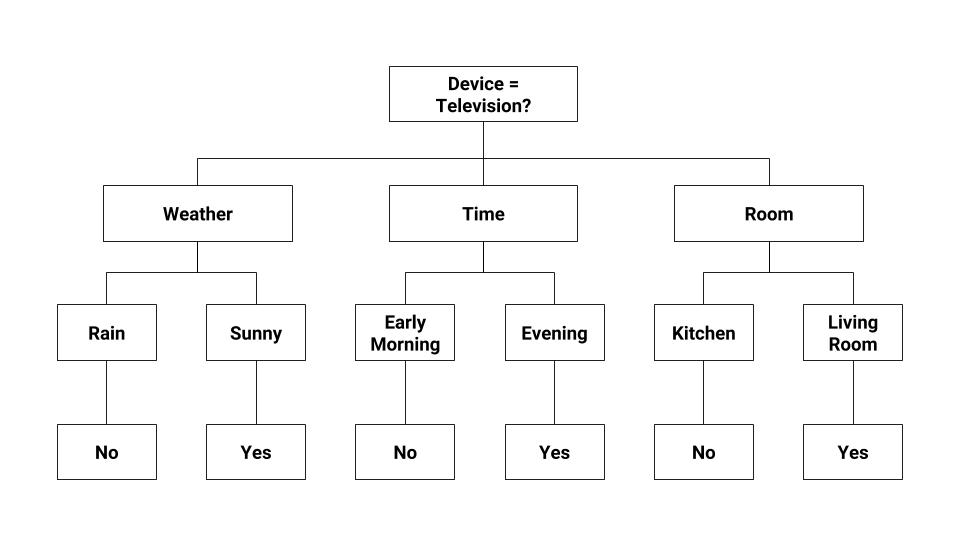
\includegraphics[scale=0.45]{images/tree.jpg}
	    \centering
	    \caption{Electricity Tariff}
	    \label{cost}
	\end{figure}


Hence in addition to the current, active power and reactive power classification parameters, we propose the use of additional parameters such as:

\subsection{Weather}
The current weather may determine the state of the device. For example, when the temperature is low and the residents begin to feel cold during the winter, the likelihood of the Air Conditioner being on is highly unlikely.
The weather data will have to be calibrated according to a particular geographic location

\subsection{Time & Day}
The time of the day can also be used to determine the state of the device. For example, during the day and during the night(sleep time 1 A.M. to 6 A.M.), the likelihood of the use of high power lighting is highly unlikely.

In some cases the day of the week can be used as an additional classification parameter. For example, during weekends, more people are present at home(weekdays spent at Work,college,etc), hence the likelihood of the use of entertainment systems such as Television and Gaming systems during the midday as well as the likelihood of the use of kitchen appliances during the midday will significantly increase. 

This may vary from household to household but with a large dataset of mixed households, this parameter may become very useful.

The time & day data will have to be calibrated according to a particular timezone.

\subsection{Room Location}
{
Certain load appliances have fixed places within an household. By creating another parameter which takes into account the location of a load appliance within the household can also improve the quality of the dataset. 
For example, most households have refrigerators & microwaves in the kitchen, water heating geysers in the bathroom, televisions & home theatre systems in the living room. On the other hand, the likelihood of an Air Conditioner within a bathroom will be highly unlikely. 

This will indeed require additional hardware and separate current sensors per room.
}

\section{Voltage Calibration}
{


\begin{figure}[H]
	    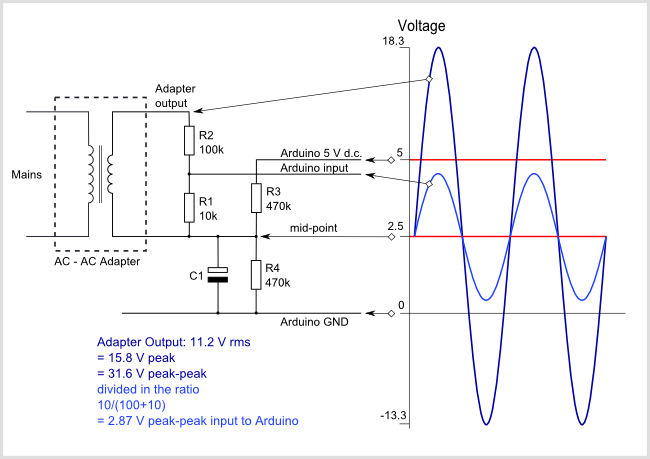
\includegraphics[scale=0.70]{images/volt.png}
	    \centering
	    \caption{Voltage Calibration}
	    \label{volt}
	\end{figure}

\begin{equation}
    Peak\ Output\ Voltage = \frac{R_1} {R_1 + R_2} \times Peak\ Input\ Voltage
\end{equation}

The standard household AC voltage provided by electricity distributors varies from 220V to 240V. 
Hence the voltage value will vary depending on the location, electricity distributor and even in some cases voltage fluctuations.
In order taken into account such voltage variations, the voltage transformer is used to calibrate the household voltage once the Smart Energy Monitor has been installed.  
}

\section{Estimating Electricity Bill}

\begin{figure}[H]
	    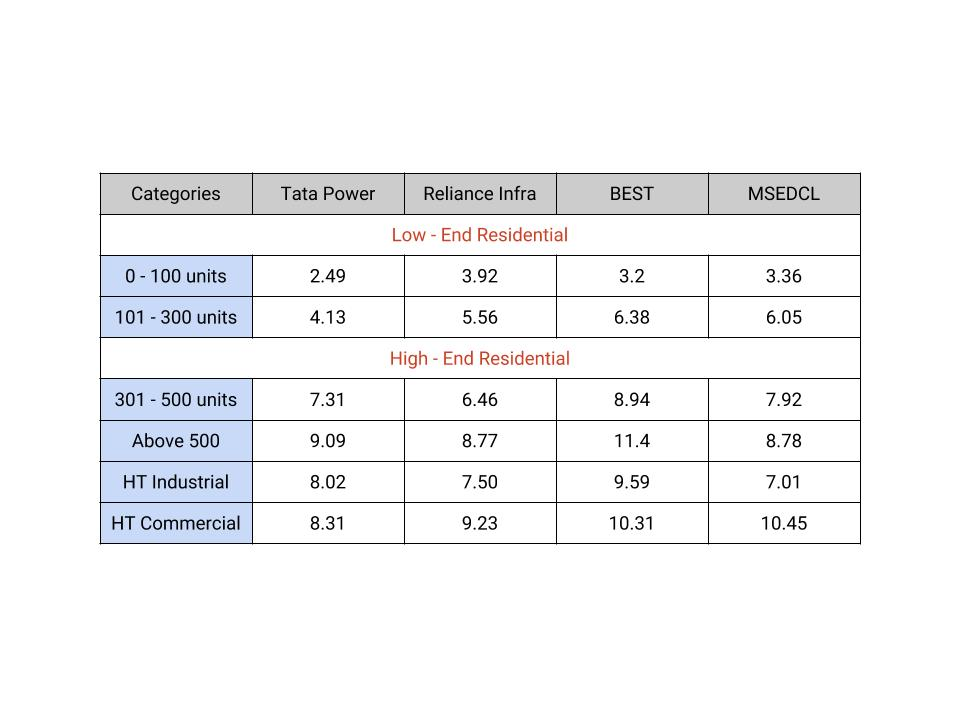
\includegraphics[scale=0.45]{images/cost.jpg}
	    \centering
	    \caption{Electricity Tariff}
	    \label{cost}
	\end{figure}

\begin{equation}
    Monthly\ Electricity\ Bill = Number\ of\ Units\ Consumed \times Cost\ per\ Unit
\end{equation}

By calculating the total number of units (1KWh = 1unit) consumed per month we can estimate the electricity bill for that month. The cost per unit of electricity will vary based on the electricity distributor as well as the number of units consumed.


\section{User Interface}
{}


\subsection{Flask Microframework}
{The user interface uses a Python Micro-Framework called Flask which is used to build web applications.

The Flask framework encodes the real time Python Variables into a JavaScript Object Notation(JSON) string.

The JSON string is then read into the HTML file using Asynchronous JavaScript And XML(AJAX) requests. 

These requests are periodically refreshed using the Auto-Refresh function in AJAX.}
\begin{figure}[H]
	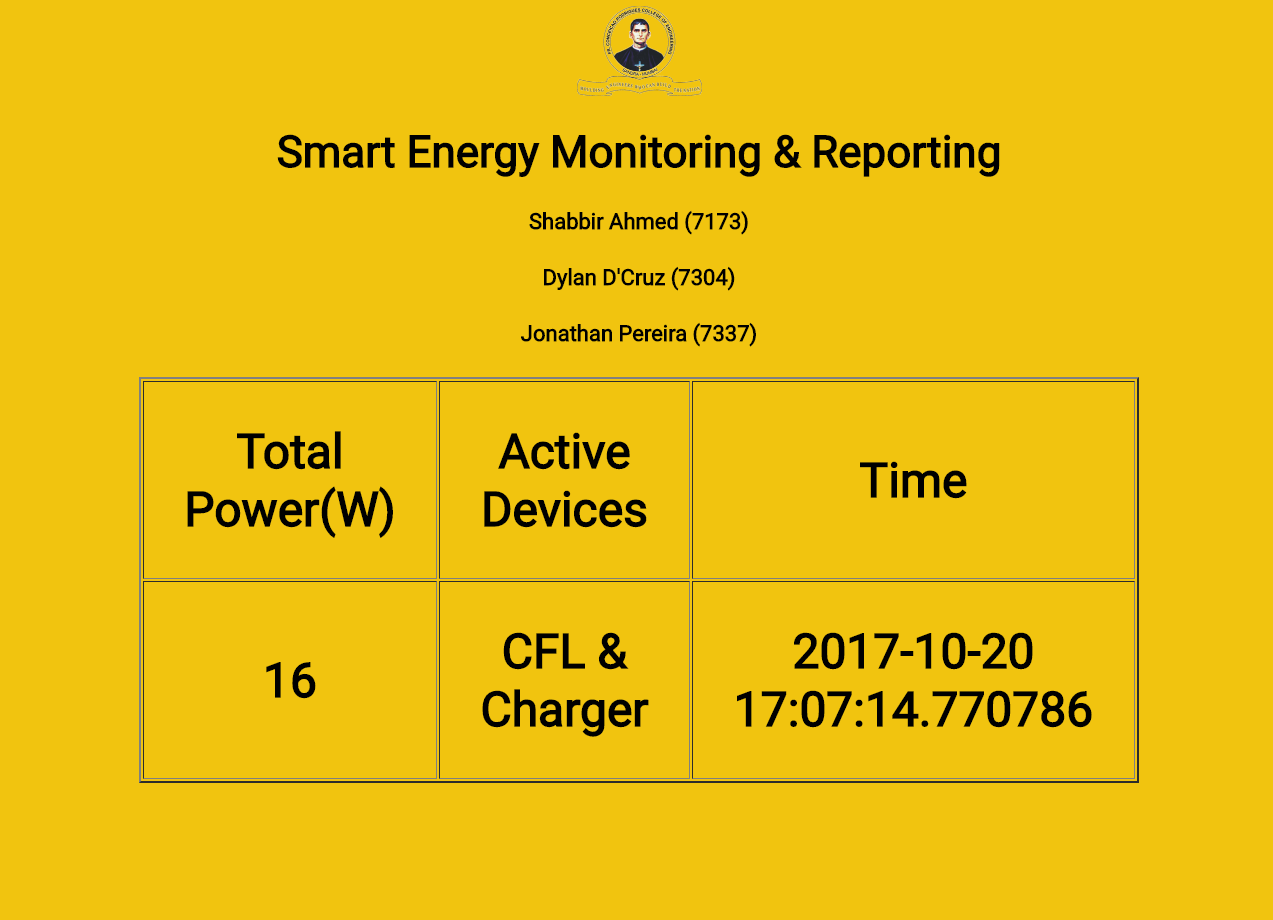
\includegraphics[width=0.9\textwidth]{Demo1.PNG} % first figure itself
	\caption{HTML-Based UI}
	\label{UI}
\end{figure}
{The user interface displays various system parameters such as Total Power being Consumed, Active Devices and the Real Time Clock. Additional parameters such as Estimated Monthly Electricity bill can be added in the future.}


\subsection{Dash Framework}{
\begin{figure}[H]
	    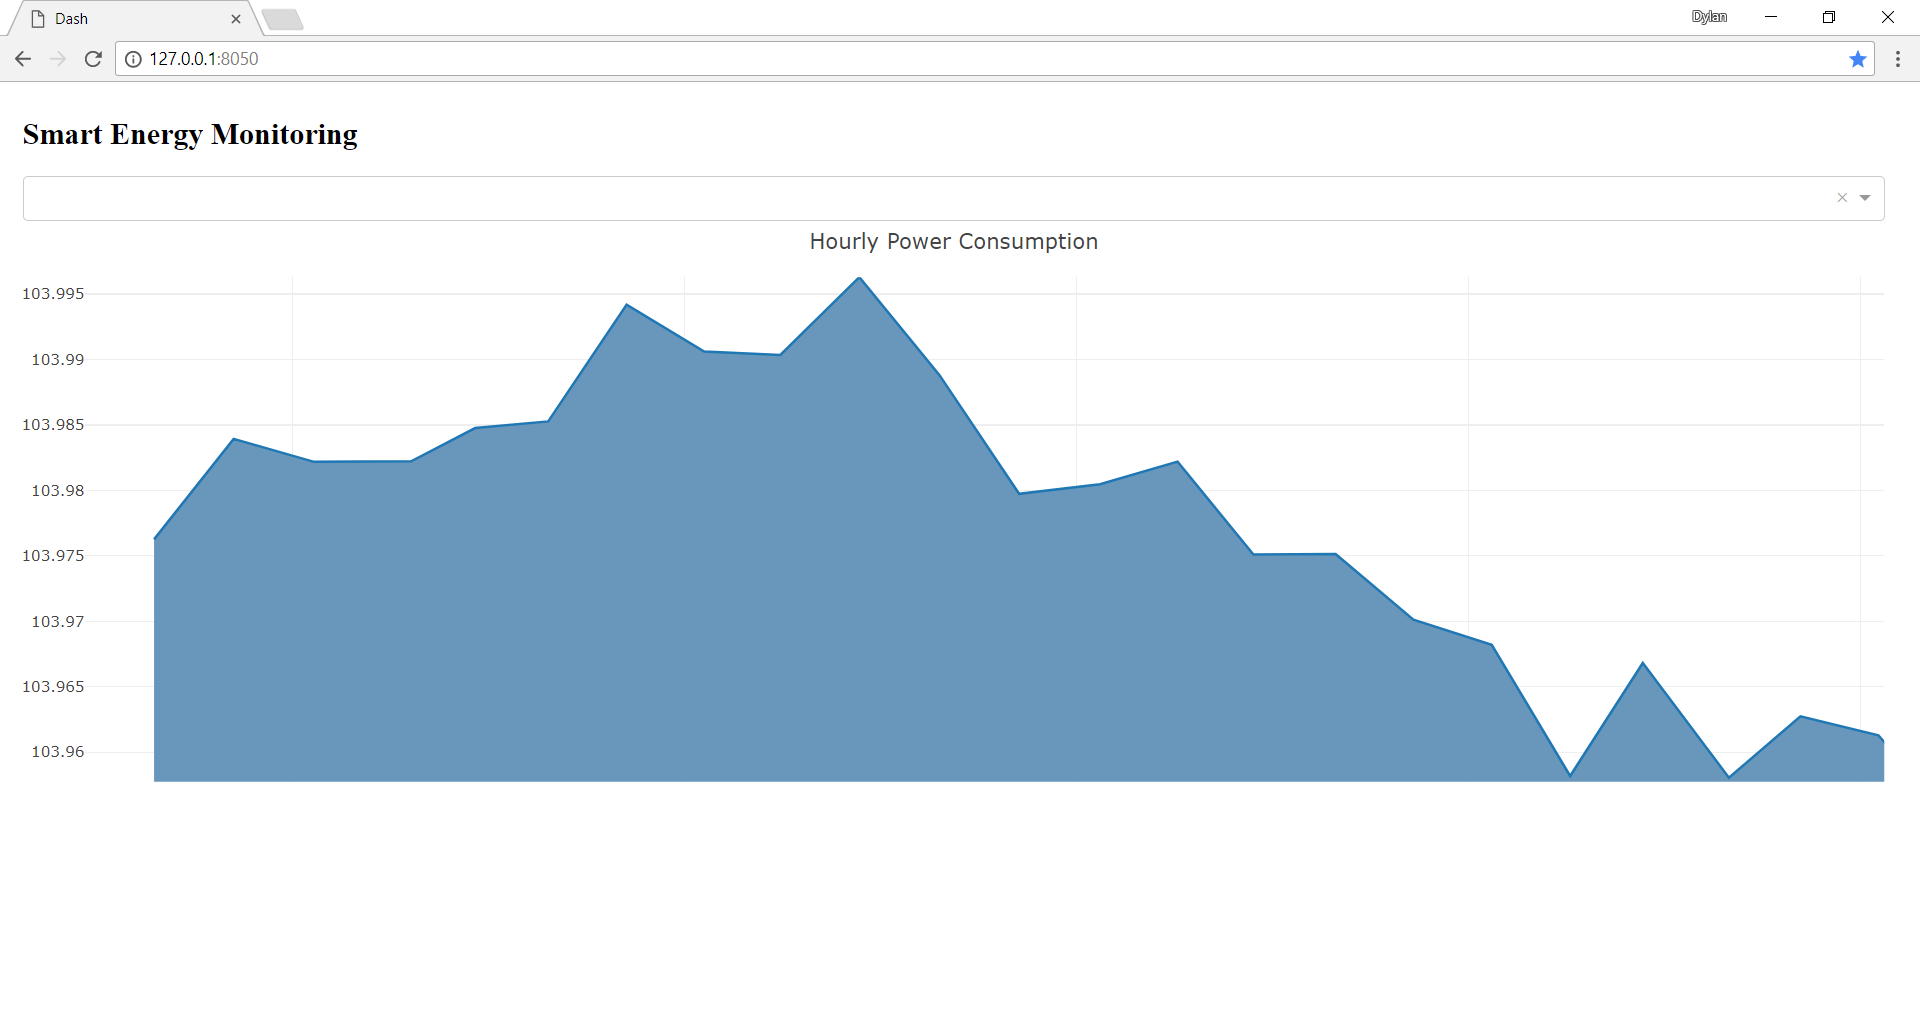
\includegraphics[scale=0.25]{images/dash.jpg}
	    \centering
	    \caption{Hourly Power Consumption over a 24hr period cycle using Dash}
	    \label{Dash}
	\end{figure}
	



Dash is a Python framework for building analytical web applications. There is no JavaScript required.
Built on top of Plotly.js, React, and Flask, Dash ties modern UI elements like dropdowns, sliders, and graphs to your analytical Python code.

We plan on using Dash to plot various live graphs as well as a pie chart of the energy usage of all load appliances.
}